\documentclass[times, utf8, diplomski, numeric]{templates/template}
\usepackage{booktabs}

\begin{document}

\sveuciliste{SVEUČILIŠTE U ZAGREBU}
\fakultet{FAKULTET ELEKTROTEHNIKE I RAČUNARSTVA}

\title{Programska podrška sustava za određivanje i upravljanje orijentacijom satelita}

\thesisnumber{2346}

\author{Ivan Vnučec}

\maketitle

% Ispis stranice s napomenom o umetanju izvornika rada. 
\izvornik

% TODO: Dodaj zahvalu
\zahvala{Josip, Karla}

\tableofcontents

% TODO: delete me
\nocite{*}

\chapter{Uvod}{
    \section{Mali sateliti}{
        %- sto su mali sateliti
        Mali sateliti su skupina satelita koji su, u usporedbi sa konvencionalnim satelitima, uvelike ograničeni prema masi, cijeni, kao i prema vremenu potrebnom da ih se razvije. Sve je to izravan rezultat revolucije u elektronici i računarstvu.\cite{hrvatskiVojnik}.

        %- tko ih koristi
        Primjene malih satelita nalazimo u svim granama svemirske industrije: u telekomunikaciji, navigaciji, opservaciji Zemlje, znanstvenim istraživanjima i dr.
        
        %- zasto ih koristimo
        Njihova zastupljenost na tržištu raste iz godine u godinu jer pružaju jeftin i brz razvoj uz relativno male tehničke zahtjeve \cite{rastMalihSatelita}. Primjenom većeg broja malih satelita povezanih u konstelaciju, moguće je primjerice pokriti veću površinu zemlje i tako stvoriti uvijek dostupni internet ili navigacijski sustav.
        
        \subsection{Podjela}{
            Iako postoje više vrsta podjela satelita u ovisnosti od izvora do izvora, navest ćemo podjelu prema FAA \engl{Federal Aviation Administration} koja uključuje satelite sa najvećom, pa sve do satelita sa najmanjom masom \cite{podjelaPremaMasi}. Podjelu je moguće vidjeti u tablici \ref{tbl:podjelaSatelita}.

            \begin{table}[htb]
            \caption{Podjela malih satelita prema masi}
            \label{tbl:podjelaSatelita}
            \centering
            \begin{tabular}{ll} \toprule
            Naziv kategorije satelita & Masa (kg) \\ \midrule
            Small & 601 - 1200 \\
            Mini & 201 - 600 \\
            Micro & 11 - 200 \\
            Nano & 1.1 - 10 \\
            Pico & 0.09 - 1 \\
            Femto & 0.01 - 0.1 \\ \bottomrule
            \end{tabular}
            \end{table}

            Maleni sateliti \engl{Small} teže manje od 1200 kilograma, cijena im je nešto manje od 30 milijuna GBP (britanskih funti) za izradu i lansiranje te je potrebno od 2 do 3 godine za njihov razvoj. Mini sateliti teže do 600 kilograma i njihov razvoj traje dvije godine po cijeni do 30 milijuna GBP. Micro sateliti su teški manje od 200 kilograma i koštaju manje od 10 milijuna GBP. Ispod te klase nalaze se Nano sateliti, težine do 10 kilograma, te Pico i Femto sateliti težine manje od 1 kilograma \cite{hrvatskiVojnik}.

            \subsubsection{Cubesat format}{
                %- sto je cubesat satelit
                %- od cega se sastoji, 
                %    - građa, 
                %    - nacin slaganja dodatnih modula
                %- kojih sve verzije cubesat satelita postoje
                %- zasto bas kocka
                %- prednosti i mane cubesat satelita
                %- navesti negdje brojke o udijelu cubesat sateltia u ostalim satelitima kroz godine
                %- zasto je popularan cubesat format
            }
        }
        
        \subsection{Metode lansiranja}{
            %- objasniti kako se sateliti lansiraju
            %    - objasni da oni nisu glavni payload
            %    - objasni kako su pakirani
            %    - objasni u koje orbite mogu ici
            %    - objasni tvrtke koje se bave lansiranjem
            %- navedi koliko najcesce kosta lansiranje
            %- navedi kako najlakse iznajmit lansiranje
            %- rast lansiranja nanosateltia iz godine u godinu
            %    - pronaci negdje neke brojke o lansiranju cubesat satelita po godinama
        }
        
        \subsection{Povijesni pregled misija}{
            %- navesti neke komercijalne primjene do sada
            %- navesti znanstvene misije do sada
        }
    }

    \section{Korisni teret satelita}{
        % sto je korisni teret satelita
        Korisni teret satelita \engl{payload} jest podsustav, ili skupina podsustava, koji imaju za cilj ispuniti zadaću koja im je dodijeljena (misija). Primjerice, ako je cilj satelita fotografiranje Zemljine površine, onda će njegov koristan teret biti sustav za fotografiranje (kamera). Ili primjerice ako želimo uspostaviti komunikaciju sa satelitom, što je gotovo uvijek slučaj, onda će njegov korisni sustav biti sustav za komunikaciju.

        \subsection{Vrste tereta}{
            %- navesti korisne terete koje satelit ima u ovisnosti o tipu misije
            Ovisno o tipu misije, razlikujemo podsustave koje je moguće svrstati u nekoliko sljedećih kategorija:

            \begin{itemize}
                \item Opservacija Zemlje
                \item Komunikacija
                \item Navigacija
                \item Znanost i tehnologija
            \end{itemize}

            Sustavi za opservaciju Zemlje sadrže uređaje koji promatraju Zemljinu površinu ili atmosferu. Najčešće takav sustav sadrži kameru koja fotografira u odabranom dijelu spektra. Zbog toga što na takvom sustavu osim kamere imamo i objektive koji omogućuju velika uvećanja, potrebno je da posjedujemo mogućnost preciznog usmjeravanja kamere. Također, sustav za komunikaciju, osim sklopovlja za obradu signala, sadrži i antene. Kako bi pospješili prijem i odašiljanje, potrebno je usmjeriti antenu prema drugoj anteni na Zemlji \cite{sattelitePayload}.

            \subsection{Važnost kontrolirane orijentacije}{
                Osim gore opisanih sustava kojima je važna kontrola orijentacije, navest ćemo još jedan primjer gdje nam je kontrola orijentacije važna. Naime, prilikom izbacivanja satelita iz samog prijevoznog sredstva u svemir, događa se nekontrolirana rotacija satelita. Kako bi satelit zaustavio rotaciju, aktivni sustav kontrolu orijentacije ulazi u posebni način rada \engl{detumbling} u kojem će zaustaviti nekontroliranu rotaciju. Takav zahvat može potrajati tjednima ili mjesecima, ovisno o tipu satelita \cite{fersat}.
            }
        }
    }
}

\chapter{Opis orijentacije satelita}{
    Kako bi matematički prikazali rotacijsko gibanje satelita, satelit je prvo potrebno modelirati kao kruto tijelo. Mi ćemo u nastavku navesti samo osnovne izraze potrebne za modeliranje satelita, a potpune matematičke izraze i izvode moguće je pronaći u popratnoj literaturi \cite{adcsKnjiga}.

    Ako govorimo o orijentaciji, važno je objasniti pojam referentnog sustava \engl{reference plane}. Referentni sustav je skup 3 međusobno ortogonalnih vektora prema kojima određujemo sve ostale vektore, bilo njihovu orijentaciju, bilo pomak. Jedan možda najpoznatiji primjer takvog referentnog sustava je Kartezijev referentni sustav gdje smo kao referentne vektore izabrali 3 jedinična vektora $\textbf{i}$, $\textbf{j}$ i $\textbf{k}$ prema kojima onda određujemo sve ostale vektore koje definiramo u Kartezijevom prostoru. 

    Moguće je imati više referentnih sustava. Prelazak iz jednog u drugi referentni sustav moguće je ostvariti transformacijama sa rotacijskim matricama o kojima ćemo govoriti kasnije. Referentne sustave najčešće označavamo kao npr. $\mathcal{F}_a$ ili $\mathcal{F}_b$. Rotacijska matrica koja bi određivala orijentaciju $\mathcal{F}_a$ referentnog sustava naspram $\mathcal{F}_b$ referentnog sustava označavamo kao $\textbf{C}_{ab}$.

    Da bi definirali orijentaciju satelita, prvo moramo definirati referentne sustave. Prvi referentni sustav kojeg definiramo je inercijski referentni sustav $\mathcal{F}_G$. U klasičnoj fizici, inercijski sustav označava referentni sustav koji ne posjeduje akceleraciju \cite{inertialFrame}. Drugi referentni sustav kojeg definiramo je tzv. \emph{body} referentni sustav $\mathcal{F}_b$ koji je nepomičan s obzirom na gibanje čvrstog tijela (satelita).

    Orijentacija satelita u referentnom sustavu $\mathcal{F}_b$ naspram inercijskog referentnog sustava $\mathcal{F}_G$ označavamo rotacijskom matricom $\textbf{C}_{bG}$.

    \section{Osnovni parametri satelita}{
        Inercijska matrica \engl{Moment of inertia tensor} u pojednostavljenom smislu označava moment tromosti krutog tijela oko pojedine osi rotacije. Naglašavamo da je u pitanju pojednostavljena definicija i da ona nije strogo točna, no za naše potrebe je ona dovoljna. Inercijsku matricu predstavljamo kao:

        \begin{equation}
        \textbf{J} = 
        \begin{bmatrix}
            J_{xx} & J_{xy} & J_{xz} \\
            J_{yx} & J_{yy} & J_{yz} \\
            J_{zx} & J_{zy} & J_{zz}
        \end{bmatrix}
        .
        \end{equation}

        Moguće je pokazati da za svako kruto tijelo možemo pojednostaviti Inercijsku matricu te tako dobiti dijagonalnu inercijsku matricu. Takva matrica nam omogućuje izvedbu jednostavnijih izraza za rotaciju krutog tijela. Zbog nepotrebnog ulaženja u detalje kako je moguće dobiti dijagonalnu matricu, navest ćemo samo izraz kao:

        \begin{equation}
        \textbf{I} = 
        \begin{bmatrix}
            I_{xx} & 0      & 0 \\
            0      & I_{yy} & 0 \\
            0      & 0      & I_{zz} \\
        \end{bmatrix}
        .
        \end{equation}
    }

    \section{Eulerovi kutovi}{
        Eulerovi kutovi predstavljaju 3 kuta između nekog vektora i ortogonalnih osi koje razapinju Kartezijev koordinatni sustav. Ako želimo predstaviti rotaciju između jednog proizvoljnog vektora i nekog drugog vektora, onda to možemo napraviti na nekoliko načina. Jedan primjer takve rotacije navest ćemo u sljedećem primjeru:

        \begin{enumerate}
            \item Rotacija za kut $\psi$ oko orginalne z-osi \engl{yaw}.
            \item Rotacija za kut $\theta$ oko tranzicijske y-osi \engl{pitch}.
            \item Rotacija za kut $\phi$ oko transformirane x-osi \engl{roll}.
        \end{enumerate}

        Uzmemo li za primjer 3 uzastopne rotacije: prve oko orginalne z-osi, zatim druge oko tranzicijske y-osi i na kraju treće oko transformirane x-osi dobivamo rotaciju prikazanu na slici ispod: 

        \begin{figure}[htb]
        \centering
        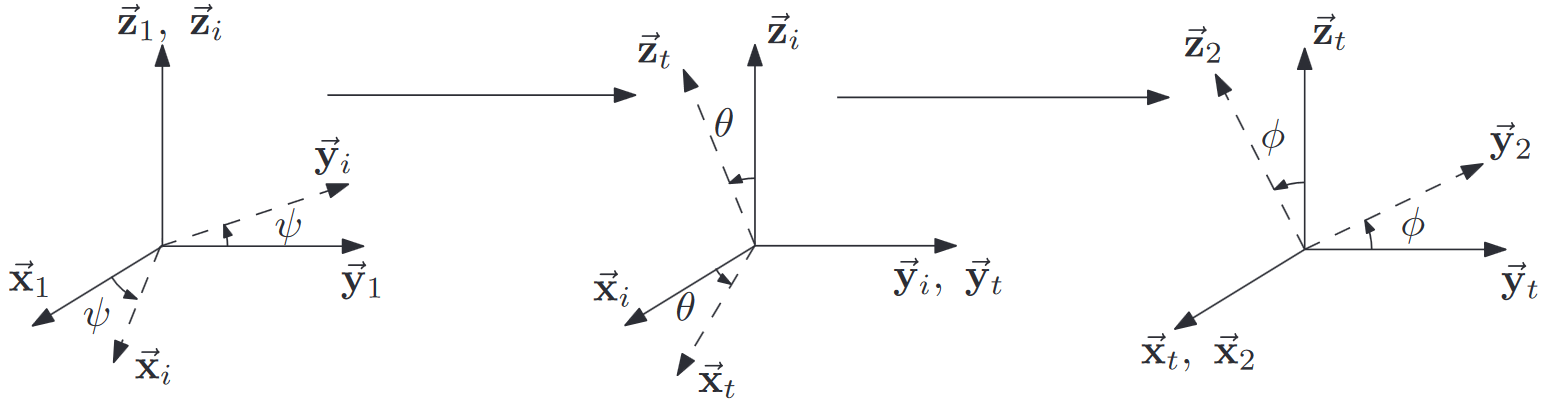
\includegraphics[width=1.0\textwidth]{images/eulerovi_kutovi.jpg}
        \caption{Tri uzastopne rotacije oko z-osi, y-osi i x-osi za kut $\psi$, $\theta$, i $\phi$}
        \label{fig:euler_rotacija}
        \end{figure}
    }

    \section{Kvaternioni}{
        Kvaternion je četvero-dimenzionalni vektor s kojim je moguće opisati orijentaciju tijela. Kvaternion u usporedbi sa Eulerovim kutovima posjeduje dvije prednosti (o kojima nešto više u nastavku): prva je da ne posjeduje singularnost, i druga da matematičke relacije modeliranja orijentacije više nisu trigonometrijske već algebarske prirode, što ih dodatno čini pogodnima za računanje.

        Kvaternion opisuje dvije stvari potrebne za opis rotacije: glavnu os rotacije \engl{principal axis} $\overrightarrow{\textbf{a}}$ i kuta rotacije $\phi$ kao što je vidljivo na slici \ref{fig:principal_axis_rotation}. Zbog toga, razlikujemo vektorski i skalarni dio koje definiramo kao:

        \begin{figure}[htb]
        \centering
        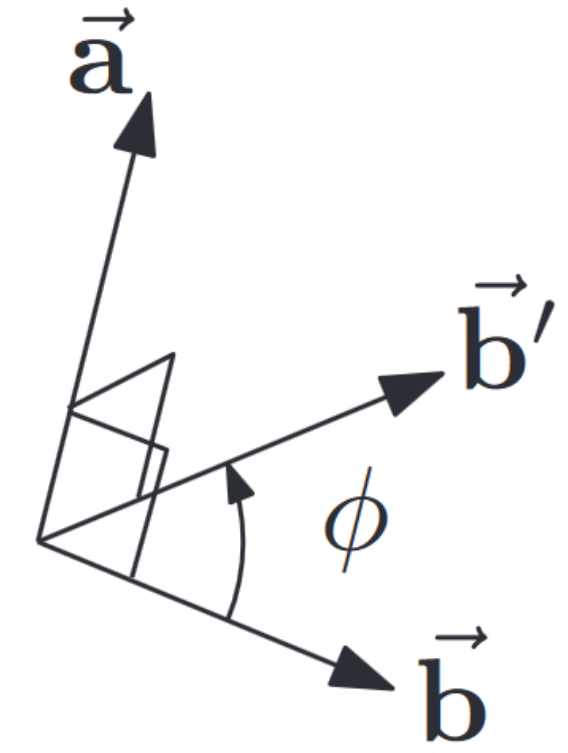
\includegraphics[width=0.2\textwidth]{images/principal_axis_rotation.png}
        % TODO: dodaj strelice iznad vektora (oprez: latex zeza nesto)
        \caption{Prikaz rotacije vektora $\textbf{b}$ oko glavne osi rotacije $\textbf{a}$ za kut $\phi$.}
        \label{fig:principal_axis_rotation}
        \end{figure}

        \begin{equation}
        \label{eq:kvaternion}
        \begin{array}{rcl}
            \boldsymbol\epsilon &  = & \overrightarrow{\textbf{a}}\sin\frac{\phi}{2} = \left[\epsilon_{x} \; \epsilon_{y} \; \epsilon_{z} \right], \\
            \eta & = & \cos\frac{\phi}{2}
        \end{array}
        \end{equation}

        U praksi postoje dvije interpretacije kvaterniona u ovisnosti o tome ide li skalarni dio kao prvi element kvaterniona ili kao posljednji. U našem radu pretpostavit ćemo oblik kvaterniona gdje je skalarni dio prvi:

        \begin{equation}
            \textbf{q}=
            \left[\eta \; \boldsymbol\epsilon \right] = \left[q_{0} \; q_{1} \; q_{2} \; q_{3}\right]
        \end{equation}
    }

    \section{Rotacijska matrica}{
        Rotacijska matrica opisuje transformaciju vektora iz orginalnog u rotirani, za neku poznatu rotaciju. U nastavku ćemo navesti rotacijske matrice koje određujemo pomoću Eulerovih kutova i pomoću kvaterniona i dati ćemo primjer rotacije vektora.

        \subsection{Prikaz pomoću Eulerovih kutova}{
            U nastavku ćemo navesti prikaze rotacijskih matrica pomoću Eulerovih kutova. Prvo ćemo navesti kako izgledaju rotacijske matrice kada imamo rotacije samo oko glavnih osi, a zatim ćemo navesti izraz za rotacijsku matricu za 3-2-1 uzastopnu rotacijsku sekvencu.

            \subsubsection{Rotacije oko glavnih osi}{
                Bez ulaženja u detalje, navest ćemo redom kako izgledaju rotacijske matrice za rotacije oko z, y i x osi. Prikaze tih rotacija moguće je vidjeti na slici \ref{fig:principal_rotations}.

                Rotacija oko z-osi:

                \begin{equation}
                \label{eq:principal_rot_z}
                \textbf{C}_{z}(\theta_{z}) = 
                \begin{bmatrix}
                    \cos\theta_{z}   & \sin\theta_{z}    &  0 \\
                    -\sin\theta_{z}  & \cos\theta_{z}    &  0 \\
                    0                & 0                 &  1
                \end{bmatrix}
                .
                \end{equation}

                Rotacija oko y-osi:

                \begin{equation}
                \label{eq:principal_rot_y}
                \textbf{C}_{y}(\theta_{y}) = 
                \begin{bmatrix}
                    \cos\theta_{y}   &    0    &  -\sin\theta_{y} \\
                    0                &    1    &  0               \\
                    \sin\theta_{y}   &    0    &  \cos\theta_{y}
                \end{bmatrix}
                .
                \end{equation}

                Rotacija oko x-osi:

                \begin{equation}
                \label{eq:principal_rot_x}
                \textbf{C}_{x}(\theta_{x}) = 
                \begin{bmatrix}
                    1    &      0           &  0 \\
                    0    & \cos\theta_{x}   &  \sin\theta_{x} \\
                    0    & -\sin\theta_{x}  &  \cos\theta_{x}
                \end{bmatrix}
                .
                \end{equation}

                \begin{figure}[htb]
                \centering
                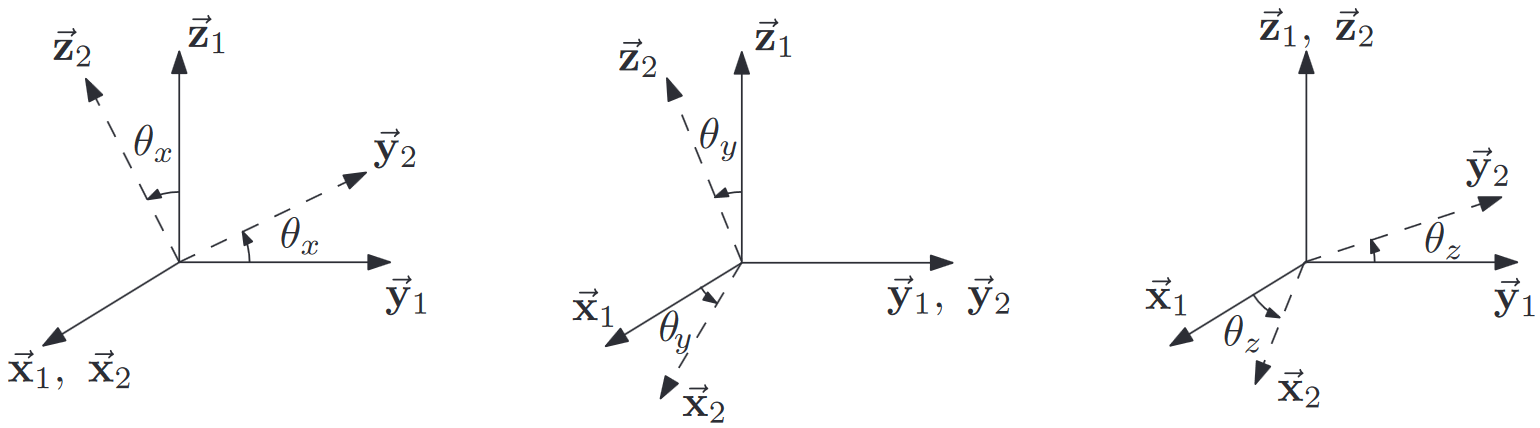
\includegraphics[width=1.0\textwidth]{images/principal_rotations.png}
                \caption{Prikaz rotacija oko glavnih osi.}
                \label{fig:principal_rotations}
                \end{figure}
            }

            \subsubsection{3-2-1 rotacijska sekvenca}{
                Rotacija sekvenca koja je jako česta u zrakoplovno-svemirskoj industriji označava se kao 3-2-1 orijentacijska sekvenca \engl{attitude sequence}. Takvo ime je uzeto zato što je prva rotacija oko orginalne z-osi (oznaka 3), zatim slijedi rotacija oko tranzicijske y-osi (oznaka 2) te na kraju rotacija oko transformirane x-osi (oznaka 1).

                3-2-1 rotacijsku matricu moguće je prikazati pomoću Eulerovih kutova kao:

                \begin{equation}
                \label{eq:euler_rot_mat}
                \begin{array}{rcl}
                \textbf{C}_{21}(\phi, \theta, \psi) & = & \textbf{C}_{x}(\phi) \textbf{C}_{y}(\theta) \textbf{C}_{z}(\psi) \\
                & = &
                \begin{bmatrix}
                    c_{\theta}c_{\psi}                            & c_{\theta}s_{\psi}                            & -s_{\theta} \\
                    s_{\phi}s_{\theta}c_{\psi} - c_{\phi}s_{\psi} & s_{\phi}s_{\theta}s_{\psi} + c_{\phi}c_{\psi} & s_{\phi}c_{\theta} \\
                    c_{\phi}s_{\theta}c_{\psi} + s_{\phi}s_{\psi} & c_{\phi}s_{\theta}s_{\psi} - s_{\phi}c_{\psi} & c_{\phi}c_{\theta}
                \end{bmatrix}
                \end{array}
                ,
                \end{equation}

                gdje radi preglednosti vrijedi $s_{b}=\sin(b)$ i $c_{b}=\sin(b)$.

                Primijetimo kako smo 3-2-1 rotacijsku matricu dobili tako što smo množili pojedinačne matrice rotacija oko glavnih osi (vidi jednadžbe \ref{eq:principal_rot_z}, \ref{eq:principal_rot_y} i \ref{eq:principal_rot_x}). Važno je napomenuti kako u ovom slučaju ne vrijedi komutativnost i da je redoslijed umnoška matrica bitan.
            }

            \subsubsection{Singularnost Eulerovih kutova}{
            \label{subsubsection:singularnost_eulerovih_kutova}
                Jedna mana reprezentacije rotacije pomoću Eulerovih kutova je tzv. singularnost. Može se pokazati da za svaku parametrizaciju rotacije može doći do singulariteta. Za naš primjer 3-2-1 sekvence singularitet nastaje kada je $\theta=\pm90^{\circ}$. Za takav slučaj rotacijska matrica postaje:

                \begin{equation}
                \textbf{C}_{21}(\phi, 90^{\circ}, \psi) =
                \begin{bmatrix}
                    0                 & 0                  & -1 \\
                    \sin(\phi - \psi) & \cos(\phi - \psi)  &  0 \\
                    \cos(\phi - \psi) & -\sin(\phi - \psi) &  0
                \end{bmatrix}
                .
                \end{equation}

                Fizikalno, zbog singulariteta prva i treća rotacija unutar 3-2-1 sekvence se odvijaju oko jedne te iste osi. U tom slučaju roll i yaw ($\phi$ i $\psi$) su zapravo jednaki kutovi i ne mogu se jednoznačno odrediti. Izvan singulariteta, moguće je jednoznačno odrediti sva tri Eulerova kuta. 
            }

            \subsubsection{Određivanje Eulerovih kutova iz rotacijske matrice}{
                Ako rotacijsku matricu označimo kao:

                \begin{equation}
                \label{eq:rotation_matrix}
                \textbf{C} =
                \begin{bmatrix}
                    c_{11} & c_{12} & c_{13} \\
                    c_{21} & c_{22} & c_{23} \\
                    c_{31} & c_{32} & c_{33} \\
                \end{bmatrix}
                ,
                \end{equation}

                iz jednadžbe \ref{eq:euler_rot_mat} moguće je odrediti Eulerove kutove kao:

                \begin{equation}
                \begin{array}{rcl}
                    \phi   & = & \tan^{-1}(c_{23}/c_{33}),\\
                    \theta & = & -\sin^{-1}(c_{13}),\\
                    \psi   & = & \tan^{-1}(c_{12}/c_{11}).
                \end{array}
                \end{equation}
            }

            \textbf{Naglašavamo kako je iznimno važno da prilikom definiranja rotacije pomoću Eulerovih kutova naglasimo o kojoj sekvenci rotacije se radi (npr. 3-2-1) jer rotacijske sekvence ne komutiraju!}
        }

        \subsection{Prikaz pomoću kvaterniona}{
            Rotacijsku matricu pomoću kvaterniona definiranog ranije u radu označavamo kao:

            \begin{equation}
                \textbf{C} = (2\eta^2-1)\textbf{1} + 2\boldsymbol\epsilon\boldsymbol\epsilon^{T}-2\eta\boldsymbol\epsilon^{\times},
            \end{equation}

            gdje je $\boldsymbol\epsilon^{\times}$ definiran kao:

            \begin{equation}
                \boldsymbol\epsilon^{\times} =
                \begin{bmatrix}
                    0 & -\epsilon_{z} & \epsilon_{y} \\
                    \epsilon_{z} & 0 & -\epsilon_{x} \\
                    -\epsilon_{y} & \epsilon_{x} & 0 \\
                \end{bmatrix}
                .
            \end{equation}

            Napominjemo da prilikom računanja rotacijske matrice kvaternion $\textbf{q}$ prvo normaliziramo na jediničnu duljinu jer tako garantiramo da množenje rotacijske matrice i vektora neće rezultirati promjenom duljine vektora, već samo promjenu smjera, a to je ono što želimo. Kvaternion normaliziramo na sljedeći način:

            \begin{equation}
                \textbf{q}_{norm} = \frac{\textbf{q}}{||\textbf{q}||} = \frac{\textbf{q}}{\sqrt{q_0^2 + q_1^2 + q_2^2 + q_3^2}}
            \end{equation}

            \subsubsection{Određivanje kvaterniona iz rotacijske matrice}{
                Pomoću rotacijske matrice definirane u jednadžbi \ref{eq:rotation_matrix} moguće je odrediti sva 4 člana kvaterniona na način da prvo odredimo skalarni član kao:

                \begin{equation}
                    \eta = \pm\frac{(\text{trace}[\textbf{C}] + 1)^{\frac{1}{2}}}{2}.
                \end{equation}

                Predznak skalarnog člana nije bitan jer on fizikalno samo označava smjer rotacije. Pozitivan ili negativan predznak daju istu rotaciju.

                Jednom kada smo odredili $\eta$, moguće je odrediti $\boldsymbol\epsilon$. Može se pokazati da za $\eta \neq 0$ vrijedi:

                \begin{equation}
                \begin{array}{rcl}
                    \epsilon_{x} & = & \frac{c_{23} - c_{32}}{4\eta}, \\
                    \epsilon_{y} & = & \frac{c_{31} - c_{13}}{4\eta}, \\
                    \epsilon_{z} & = & \frac{c_{12} - c_{21}}{4\eta}.
                \end{array}
                \end{equation}

                Za slučaj kada je $\eta=0$, vrijedi da je kut zakretanja jednak $\phi=\pm\pi$. Da se pokazati da je moguće izračunati elemente $\boldsymbol\epsilon$ vektora kao:

                \begin{equation}
                \begin{array}{rcl}
                    |\epsilon_{x}| & = & (\frac{c_{11} + 1}{2})^{\frac{1}{2}}, \\
                    |\epsilon_{y}| & = & (\frac{c_{22} + 1}{2})^{\frac{1}{2}}, \\
                    |\epsilon_{z}| & = & (\frac{c_{33} + 1}{2})^{\frac{1}{2}}.
                \end{array}
                \end{equation}

                Za odabir predznaka svakog elementa $\boldsymbol\epsilon$ vektora čitatelja se savjetuje da pogleda u izvor \cite{adcsKnjiga}.
            }
        }

        \subsection{Rotacija vektora pomoću rotacijske matrice}{
            U nastavku ćemo navesti izraze za rotaciju vektora pomoću rotacijskih matrica. Prvi primjer se odnosi na rotaciju oko z-osi, a drugi primjer se odnosi na 3-2-1 rotaciju. 

            Naglašavamo kako će rotacija biti izvedena u istom referentnom sustavu i nećemo se baviti transformacijama iz jednom u drugi koordinatni sustav. Za potrebe transformacija koordinatnih sustava čitatelj se upućuje na izvor \cite{adcsKnjiga}.

            \subsubsection{Rotacija oko z-osi}{
                Ako želimo vektor $\overrightarrow{\textbf{v}}=\left[ x \; y \; z \right]^T$ rotirati oko npr. z-osi za 30 stupnjeva, prvo određujemo rotacijsku matricu pomoću jednadžbe \ref{eq:principal_rot_z} kao:

                \begin{equation}
                \textbf{C}_{z}(30^{\circ}) = 
                \begin{bmatrix}
                    \cos30^{\circ}   & \sin30^{\circ}    &  0 \\
                    -\sin30^{\circ}  & \cos30^{\circ}    &  0 \\
                    0                & 0                 &  1
                \end{bmatrix}
                ,
                \end{equation}

                zatim pomnožimo vektor $\overrightarrow{\textbf{v}}$ i matricu $\textbf{C}_{z}$ da dobijemo rotirani vektor $\overrightarrow{\textbf{v}}'$:

                \begin{equation}
                \begin{array}{rcl}
                    \overrightarrow{\textbf{v}}' & = & \textbf{C}_{z}(30^{\circ}) \overrightarrow{\textbf{v}} \\
                    & = &
                \begin{bmatrix}
                    \cos30^{\circ}   & \sin30^{\circ}    &  0 \\
                    -\sin30^{\circ}  & \cos30^{\circ}    &  0 \\
                    0                & 0                 &  1
                \end{bmatrix}
                \begin{bmatrix}
                    x \\
                    y \\
                    z
                \end{bmatrix}
                \end{array}
                .
                \end{equation}
            }

            \subsubsection{3-2-1 rotacija}{
                Ako želimo vektor $\overrightarrow{\textbf{v}}$ definiran u prošlom primjeru rotirati prvo oko z-osi za 30 stupnjeva, tranzicijske y-osi za 20 stupnjeva i na kraju oko transformirane x-osi za 10 stupnjeva, prvo određujemo rotacijsku matricu pomoću jednadžbe \ref{eq:euler_rot_mat} kao:

                \begin{equation}
                \textbf{C}_{21}(10^\circ, 20^\circ, 30^\circ) = \textbf{C}_{x}(10^\circ) \textbf{C}_{y}(20^\circ) \textbf{C}_{z}(30^\circ),
                \end{equation}

                zatim pomnožimo vektor $\overrightarrow{\textbf{v}}$ i matricu $\textbf{C}_{21}$ da dobijemo rotirani vektor $\overrightarrow{\textbf{v}}'$:

                \begin{equation}
                    \overrightarrow{\textbf{v}}' = \textbf{C}_{21}(10^\circ, 20^\circ, 30^\circ) \overrightarrow{\textbf{v}}.
                \end{equation}
            }
        }
    }

    \section{Jednadžba rotacijskog gibanja}{
        Ako govorimo o jednadžbi rotacije satelita, važno se prisjetiti definicija tzv. \emph{body} $\mathcal{F}_b
        $ i inercijskog referentnog sustava $\mathcal{F}_G$. Orijentaciju između ta dva referentna sustava moguće je opisati orijentacijskom matricom $\textbf{C}_{bG}$ i to na barem dva načina: pomoću Eulerovih kutova ili pomoću kvaterniona kao što je opisano u prethodnim poglavljima.

        Kako je $\mathcal{F}_b$ referentni sustav nepomičan s obzirom na tijelo satelita, kutnu brzinu \emph{body} referentnog sustava $\mathcal{F}_b$ s obzirom na $\mathcal{F}_G$ inercijskog sustava označavamo kao $\boldsymbol{\omega}_{bG}=\left[ \omega_1 \; \omega_2 \; \omega_2\right]^T$.

        \subsection{Prikaz pomoću Eulerovih kutova}{
            Jednadžbu rotacijskog gibanja pomoću Eulerovih kutova definiramo kao umnožak 3-2-1 rotacijske sekvence i kutne brzine kao:

            \begin{equation}
                \begin{bmatrix}
                    \dot{\phi} \\
                    \dot{\theta} \\
                    \dot{\psi}
                \end{bmatrix}
                =
                \begin{bmatrix}
                    1 & \sin\phi\tan\theta & \cos\phi\tan\theta \\
                    0 & \cos\phi & -\sin\phi \\
                    0 & \sin\phi\sec\theta & \cos\phi\sec\theta
                \end{bmatrix}
                \boldsymbol{\omega}_{bG}.
            \end{equation}
        }

        \subsection{Prikaz pomoću kvaterniona}{
            Jednadžbu rotacijskog gibanja pomoću kvaterniona i kutne brzine definiramo kao:

            \begin{equation}
            \begin{array}{rcl}
                \dot{\boldsymbol\epsilon} &  = & \frac{1}{2}(\eta\textbf{1} + \boldsymbol{\epsilon}^\times)\boldsymbol{\omega}_{bG}, \\
                \dot{\eta} & = & -\frac{1}{2}\boldsymbol{\epsilon}^T\boldsymbol{\omega}_{bG}.
            \end{array}
            \end{equation}
        }
    }

    \section{Usporedba Eulerovih kutova i kvaterniona}{
        Kao što smo već pisali u poglavlju \ref{subsubsection:singularnost_eulerovih_kutova}, dva su problema prikazivanja orijentacije pomoću Eulerovih kutova. Prvi problem je singularitet, gdje za neke kutove koje reprezentiraju istu orijentaciju (vidi poglavlje \ref{subsubsection:singularnost_eulerovih_kutova}) nije moguće jednoznačno odrediti Eulerove kutove iz rotacijske matrice. Drugi problem je što za opisivanje orijentacije koristimo trigonometrijske funkcije koje je teže izračunati na računalima nego primjerice algebarske.

        Prikaz orijentacije kvaternionom rješava nas problema singulariteta zbog dodatnog četvrtog člana. Kvaternionom smo također riješili problem računanja trigonometrijskih funkcija jer jednadžbe sa kvaternionima su algebarskog tipa.

        Pozitivna strana prikaza orijentacije pomoću Eulerovih kutova je njihova intuitivnost jer svaki kut označava kut orijentacije oko pojedine osi. Kod kvaterniona informacija o orijentaciji je ponešto sakrivena unutar kvaterniona. Skalarni član ne označava direktno kut zakreta oko osi rotacije već njegov kosinus kuta, a vektorski dio sadrži skaliranu os rotacije sinusom kuta (vidi jednadžbu \ref{eq:kvaternion}).
    }
}

\chapter{Sustav za određivanje i upravljanje orijentacijom satelita (ADCS)}{
    U ovom poglavlju navest ćemo definiciju ADCS \engl{Attitude Determination and Control system} sustava. Navest ćemo osnovne dijelove sustava. Navest ćemo najčešće korištene senzore i aktuatore, objasnit njihove karakteristike, navest prednosti i mane. Također ćemo opisati načine i algoritme određivanja i kontrole orijentacije. Naposlijetku ćemo opisati sklopovlje koje smo razvili i navesti korištene senzore i aktuatore. 

    \section{Uvod}{
        ADCS  sustav je sustav koji određuje orijentaciju satelita pomoću podataka iz senzora koji se nalaze na samom satelitu i na temelju tih podataka vrši korekciju orijentacije u željeni položaj. 

        \subsection{Određivanje i upravljanje orijentacijom}{
            Senzori koje koristi ADCS sustav za određivanje orijentacije najčešće ne daju direktno vrijednost orijentacije već se orijentacija estimira pomoću estimacijskih algoritama. Problem senzora općenito je njihova neodređenost koja onda doprinosi da je estimacija orijentacije pogrešna. Zbog toga smo razvili estimacijske algoritme koje uzimaju grešku senzora u obzir te tako smanjuju neodređenost estimirane orijentacije.

            Nakon što smo odredili orijentaciju, i ako ta orijentacija nije jednaka željenoj, slijedi postupak korekcije (kontrole). Postupak korekcije počinje računanjem razlike željene orijentacije i trenutno estimirane. Regulator orijentacije će pomoću te razlike orijentacije izračunati optimalnu korekciju koju je potrebno izvršiti kako bi došli u željenu orijentaciju. Korekciju orijentacije izvršavaju mehanički odnosno električni aktuatori. Aktuatori će stvoriti korekcijski moment koji satelit naposlijetku dovodi u željenu orijentaciju.
            Opisana estimacija i kontrola orijentacije ADCS sustava događa se u stvarnom vremenu kroz cijeli radni vijek satelita i ni u jednom trenu se ne smije dogoditi da satelit posjeduje neželjenu ili nekontroliranu orijentaciju jer to može značiti kraj misije.
        }

        \subsection{Važnost ADCS sustava}{
            NASA-ino istraživanje je pokazalo da je ADCS sustav zaslužan za 23\% grešaka na navigacijsko-kontrolnim sustavima \engl{Guidance, Navigation and Control - GN\&C}, i da je većina tih anomalija uzrokovala kraj misije \cite{greskeNaAdcsPostotak}. U nastavku ćemo navest jedan primjer greške na ADCS sustavu.
    
            Lewis svemirska letjelica \cite{lewis} lansirana je 1997. godine s predviđenim radnim vijekom od 5 godina. Nakon postizanja uspješne orbite satelit je započeo sa normalnim radom i nije ga više bilo potrebno aktivno kontrolirati. U normalnom radu solarni paneli su bili upereni prema Suncu kako bi prikupili maksimalnu količinu energije. Zbog greške prilikom rada, jedan od aktuatora je stvarao konstantni moment oko jedne osi koju senzori nisu mogli prepoznati. Nakon nekoliko dana, satelit se je počeo nekontrolirano rotirat i solarni paneli nisu prikupljali dovoljno energije. Naposlijetku su inženjeri sa Zemlje uočili nekontroliranu orijentaciju ali je već bilo kasno jer se je baterija satelita potpuno ispraznila i komunikacija sa satelitom je bila zauvijek prekinuta \cite{greskeNaAdcsSlucajevi}.
        }
    }

    \section{Osnovni dijelovi}{
        Osnovni dijelovi ADCS sustava su računalo, senzori i aktuatori. U nastavku ćemo zasebno opisati svaki dio zasebno i navesti neke važne karakteristike.
 
        \subsection{Računalo}{
            Računalo je zaslužno za prikupljanje i obradu podataka koje dolaze sa senzora, te kontrolu aktuatora. Prikupljanje podataka sa senzora vrši se preko komunikacijskih kanala (sabirnica). Obrada podataka se u suštini zasniva na računanju zahtjevnih matematičkih operacija koje na koncu daju podatak o trenutnoj orijentaciji. Na temelju razlike trenutne i željene orijentacije, računalo će izračunati kontrolni signal koji šalje aktuatorima također preko predviđenih sabirnica. 

            Neki od zahtjeva za ADCS računala su mala potrošnja, otpornost na radijaciju i kozmičke zrake, brzina izvođenja operacija, pouzdanost. U prilog ide i ako je računalo već korišteno u nekim prijašnjim misijama.
        }

        \subsection{Senzori orijentacije}{
            Senzori orijentacije su elektroničke naprave iz kojih je moguće dobiti podatak o orijentaciji. Podatak o orijentaciji najčešće ne dolazi direktno iz senzora već se orijentacija estimira matematičkim algoritmima koji kao svoj rezultat daju estimiranu orijentaciju \cite{adcsKnjiga}. Za precizno određivanje orijentacije nekada je potrebno uzeti u obzir podatke iz više senzora odjednom. Takav način prikupljanja podataka zovemo engl. \emph{sensor fusion}. 

            U nastavku ćemo navesti najkorištenije senzore, njihove karakteristike i način rada.

            \subsubsection{Senzor Sunca}{
                Senzore Sunca dijelimo u dvije skupine: analogne i digitalne. Analogni senzori Sunca rade na principu solarnih ćelija, a podatak o vektoru sunca moguće je dobiti iz generirane struje ćelija. Slika \ref{fig:sensor_sunca_industrija} prikazuje industrijsku izvedbu jednog takvog senzora.

                \begin{figure}[htb]
                \centering
                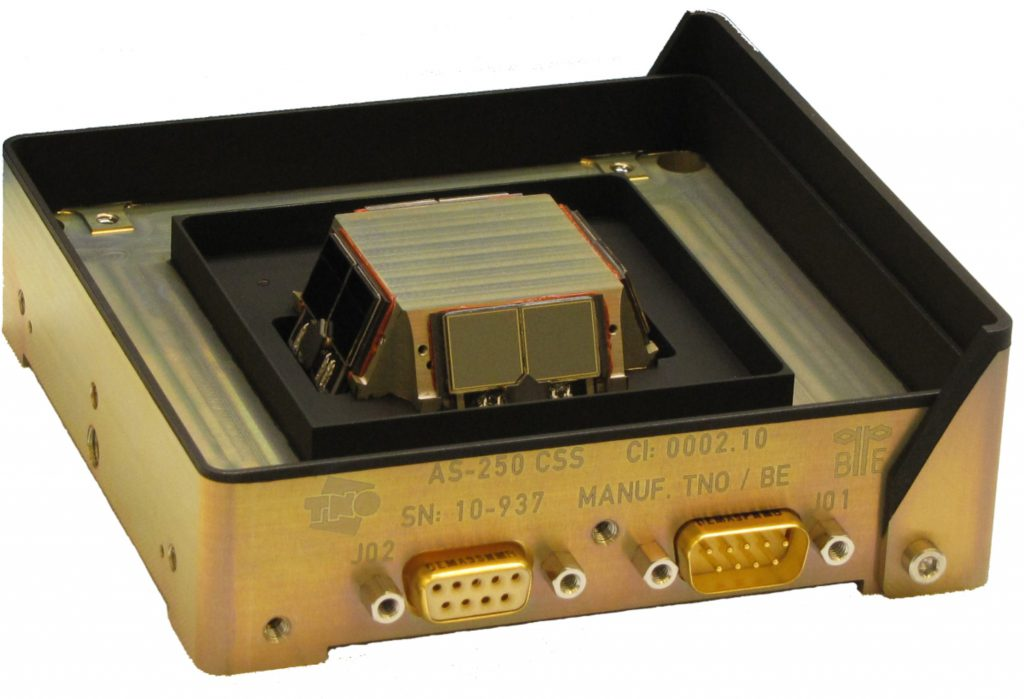
\includegraphics[width=0.6\textwidth]{images/sensor_sunca_industrija.jpg}
                \caption{Prikaz industrijske izvedbe senzora Sunca tvrtke Bradford \cite{sunSensorBradford}.}
                \label{fig:sensor_sunca_industrija}
                \end{figure}

                Struja iz solarnih ćelija ovisna je o kutu $\theta$ što označava kut između normale senzora $\hat{\overrightarrow{\textbf{n}}}$ i vektora nadolazeće zrake Sunca $\hat{\overrightarrow{\textbf{v}}}$ (vidi sliku \ref{fig:sensor_sunca}) kao:

                \begin{equation}
                    i(\theta) = i(0)\cos\theta,
                \end{equation}

                Senzor Sunca ima konačni kut gledanja u obliku stošca. Sa samo jednim senzorom Sunca nije moguće odrediti vektor $\hat{\overrightarrow{\textbf{v}}}$ već se primjenjuje paradigma \emph{sensor fusion}-a gdje koristimo dodatni senzor Sunca (vidi sliku \ref{fig:sensor_sunca_sensor_fusion}) \cite{adcsKnjiga}.

                \begin{figure}[htb]
                \centering
                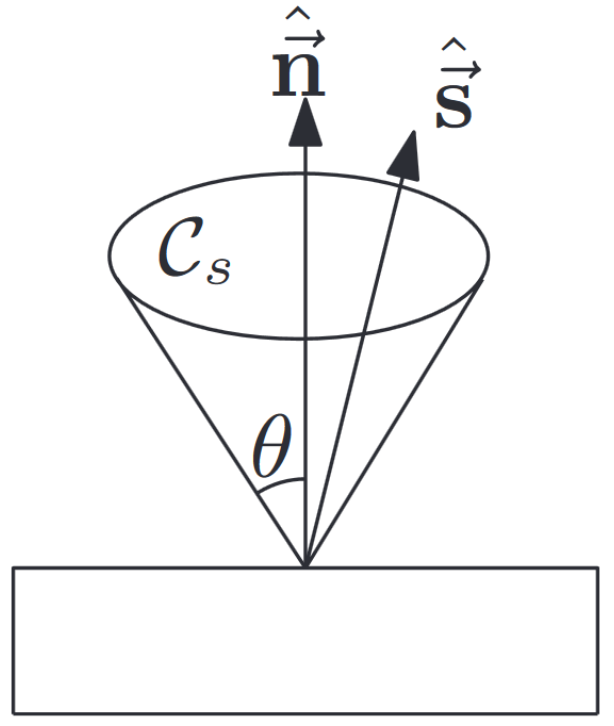
\includegraphics[width=0.3\textwidth]{images/sensor_sunca.png}
                \caption{Prikaz modela senzora Sunca.}
                \label{fig:sensor_sunca}
                \end{figure}

                \begin{figure}[htb]
                \centering
                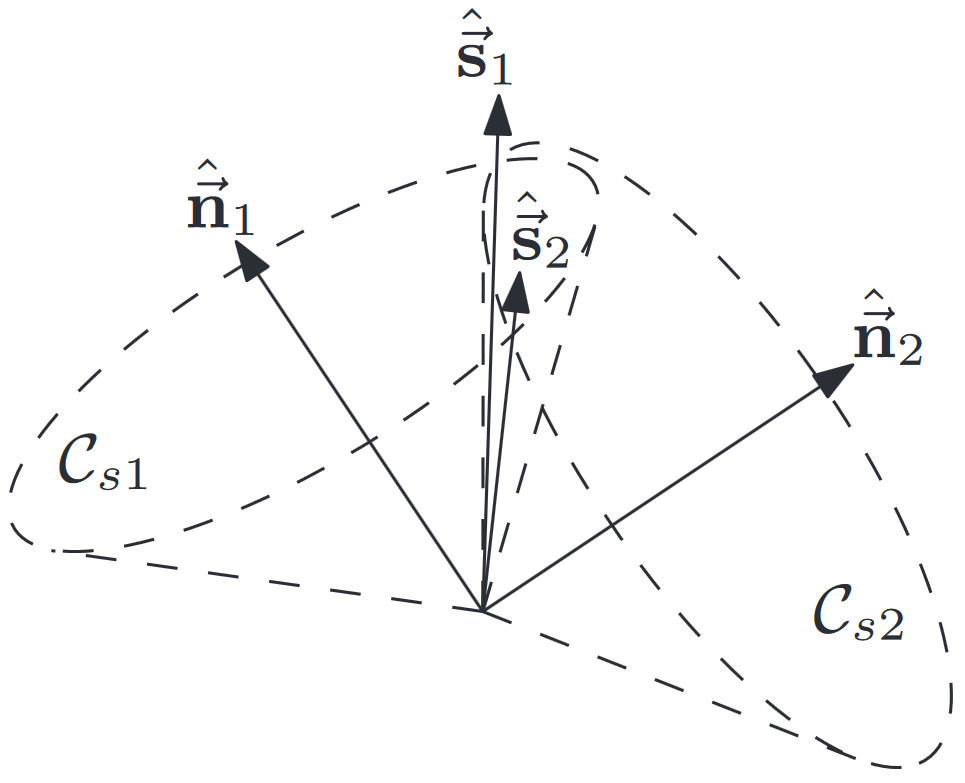
\includegraphics[width=0.55\textwidth]{images/sensor_sunca_sensor_fusion.png}
                \caption{Prikaz para senzora Sunca.}
                \label{fig:sensor_sunca_sensor_fusion}
                \end{figure}
            }

            \subsubsection{Troosni magnetometar}{
            \label{subsubsection:troosni_magnetometar}
                Troosni magnetometar mjeri vektor lokalnog magnetskog polja Zemlje u koordinatnom sustavu senzora. Magnetometri su relativno neprecizni senzori i za pouzdanija mjerenja potrebno ih je kalibrirati \cite{adcsKnjiga}.

                Kalibracija ima za cilj smanjiti utjecaj tzv. engl. \emph{Hard} i \emph{Soft} efekata. Prije nego objasnimo što su spomenuti efekti, važno je objasniti postupak kalibracije magnetometra. 

                Kalibracija magnetometra započinje prikupljanjem podataka iz senzora i to tako što ćemo magnetometar rotirati u svim smjerovima. Nakon što smo prikupili dovoljno podataka možemo prikazati izmjerene vektore magnetskog polja kao skupinu točaka gdje svaka točka prikazuje vrh vektora očitane vrijednosti. Prikaz očitanih vrijednosti kod idealnog magnetometra biti će raspoređeni po sferi radijusa duljine vektora (apsolutna vrijednost magnetskog polja) čije središte leži u centru koordinatnog sustava (vidi sliku \ref{fig:mag_ideal}).

                \begin{figure}[htb]
                \centering
                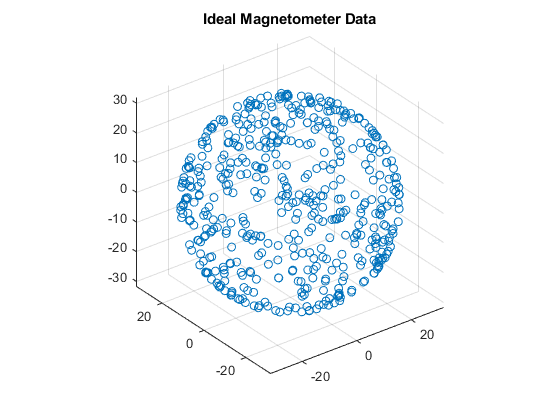
\includegraphics[width=0.7\textwidth]{images/mag_ideal.png}
                \caption{Točkasti prikaz mjerenja vektora Zemljinog magnetskog polja pomoću idealnog magnetometra. Vrijednosti mjerenja su u jedinici $\mu T$.}
                \label{fig:mag_ideal}
                \end{figure}

                Nakon što smo objasnili postupak prikupljanja podataka slijedi objašnjenje \emph{Hard} i \emph{Soft} efekata. \emph{Hard} efekt je pojava koja utječe na na mjerenja magnetskog polja i manifestira se kao translacija ishodišta svih vrijednosti mjerenog vektora magnetskog polja za neki fiksni vektor (vidi sliku \ref{fig:mag_hard}). Mogli bismo slobodno reći da su mjerenja pristrana, odnosno imaju tzv. engl. \emph{bias}. Uzrok \emph{Hard} efekta su najčešće stacionarne interferencije okolnih metalnih dijelova na samom magnetometru ili pripadajućoj elektronici. 

                \begin{figure}[htb]
                \centering
                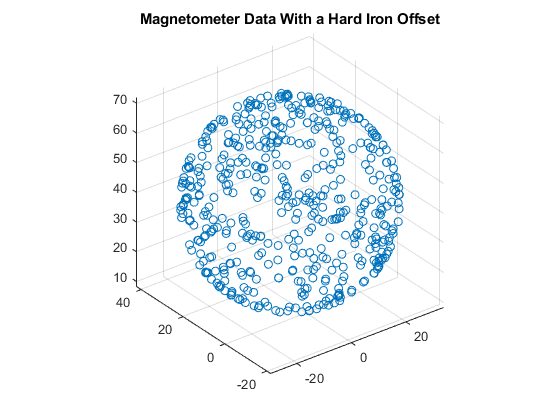
\includegraphics[width=0.7\textwidth]{images/mag_hard.png}
                \caption{Točkasti prikaz mjerenja vektora Zemljinog magnetskog polja pomoću magnetometra sa tzv. \emph{Hard} efektom. Vrijednosti mjerenja su u jedinici $\mu T$.}
                \label{fig:mag_hard}
                \end{figure}

                \emph{Soft} efekti nastaju zbog objekata u blizini magnetometra koji onda rade distorziju lokalnog magnetskog polja. \emph{Soft} efekt kolokvijalno rečeno razvlači i kosi sferu mjerenja koja zatim oblikom postaje nakošeni elipsoid (vidi sliku \ref{fig:mag_hard_soft}).

                \begin{figure}[htb]
                \centering
                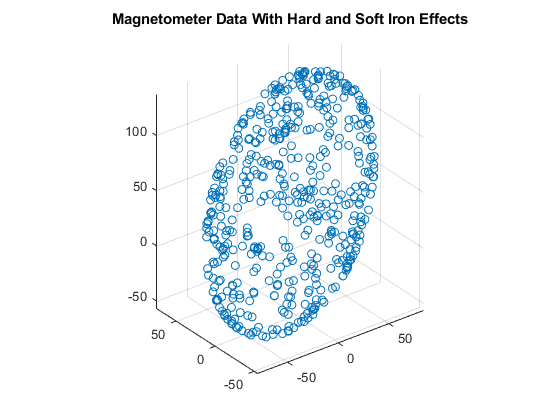
\includegraphics[width=0.7\textwidth]{images/mag_hard_soft.png}
                \caption{Točkasti prikaz mjerenja vektora Zemljinog magnetskog polja pomoću magnetometra sa tzv. \emph{Hard} i \emph{Soft} efektima. Vrijednosti mjerenja su u jedinici $\mu T$.}
                \label{fig:mag_hard_soft}
                \end{figure}

                Modeliranje spomenutih efekata opisujemo u sljedećoj jednadžbi:

                \begin{equation}
                    (x - b)R(x - b)^T = \beta^2,
                \end{equation}

                gdje je $R$ matrica tipa $3\times3$ i određuje oblik elipsoida (npr. za sferu jedinična matrica, a za elipsoid pozitivno definitna). $b$ je $1\times3$ vektor koji definira središte elipsoida, a $\beta$ je skalar koji opisuje duljinu vektora magnetskog polja. 

                Kalibracija magnetometra vrši se pomoću sljedeće relacije:

                \begin{equation}
                    m = (x - b)A,
                \end{equation}

                gdje A matrica tipa $3\times3$ transformira oblik elipsoida u pravilnu sferu (eliminira utjecaj \emph{Soft} efekta), a već definirani vektor $b$ translatira elipsoid u ishodište koordinatnog sustava (eliminira utjecaj \emph{Hard} efekta).

                Problem pronalaska $A$ i $b$ parametra rješavamo pomoću \texttt{magcal} MATLAB funkcije \cite{magcal}, a kalibraciju vršimo u programskom kodu netom nakon primitka nekalibrirane vrijednosti sa magnetometra \cite{kalibracijaMagKod}.

                Dodatna objašnjenja u vezi kalibracije magnetometra možete pronaći ovdje \cite{kalibracijaMatlabStranica}.

                Zbog vanjskog utjecaja na vrijednosti mjerenja magnetometra, magnetometar se može fizički udaljiti od satelita pomoću konstrukcije nazvane engl. \emph{boom} (vidi sliku \ref{fig:boom}) te tako smanjiti pogreške mjerenja \cite{adcsKnjiga}. 

                \begin{figure}[htb]
                \centering
                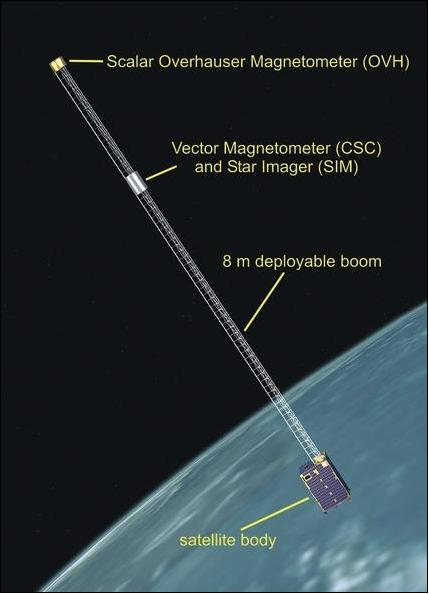
\includegraphics[width=0.5\textwidth]{images/boom.jpg}
                \caption{Prikaz tzv. \emph{boom}-a na čijem vrhu se nalazi magnetometar. Izvor Ørsted misija \cite{boomCite}.}
                \label{fig:boom}
                \end{figure}
            }

            \subsubsection{Pratioci zvijezda \engl{Star Trackers}}{
                Pratioci zvijezda odnosno \emph{Star Track}-eri pružaju najpreciznija mjerenja orijentacije iz dva razloga: prvi je što su svjetlosni izvori zvijezda točkaste prirode i tako pružaju precizna mjerenja. Drugi razlog je taj što se zvijezde, zbog svoje udaljenosti od senzora, doimaju stacionarne neovisno o položaju satelita unutar sunčevog sustava (čak i šire).

                \begin{figure}[htb]
                \centering
                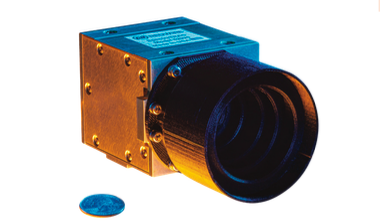
\includegraphics[width=0.5\textwidth]{images/star_tracker.png}
                \caption{Prikaz tzv. \emph{boom}-a na čijem vrhu se nalazi magnetometar. Izvor Redwire \cite{starTrackerCite}.}
                \label{fig:star_tracker}
                \end{figure}

                Pratioci zvijezda mogu pratiti vektor smjera jedne zvijezde, i u ovisnosti o položaju senzora na satelitu, orijentacijskom matricom moguće dobiti podatak smjera zvijezde u referentnom sustavu satelita. Pomoću dodatnih senzora moguće je jednoznačno odrediti orijentaciju satelita. 

                U praksi pratioci zvijezda prate više zvijezda odjednom i pomoću zvjezdanih kataloga \cite{starCatalogs} određuje direktno podatak o orijentaciji. Jednom kada je senzor odredio orijentaciju, svako sljedeće mjerenje zasniva se na praćenju istih zvijezda i metodom usrednjavanja moguće je postignuti veću preciznost. 

                Zbog navedenih razloga, pratioci zvijezda su najprecizniji senzori orijentacije od svih do sad navedenih senzora. S druge strane su i najkompleksniji, najskuplji i najnepouzdaniji senzori \cite{adcsKnjiga}. 
            }
        }

        \subsection{Senzori kutne brzine}{
            Senzori kutne brzine mjere kutnu brzinu satelita. Kao što ćemo vidjeti u nastavku rada, većina algoritama za procjenu orijentacije koriste kutnu brzinu kao dodatnu informaciju. Kutna brzina može se izračunati kao vremenska derivacija orijentacije, ali takav izračun unosi neodređenost u obliku šuma. Senzori kutne brzine nemaju izražen šum, ali zato imaju problem sa tzv. \emph{bias}-om - konstantnoj srednjoj vrijednosti koja unosi grešku u račun. 

            Osim niskog šuma, druga prednost senzora kutne brzine je što ne zahtijevaju eksterni izvor informacije. Primjerice, senzor Sunca uvijek mora imati prisutno Sunce ne bi li izračunali orijentaciju satelita. U tim situacijama kada ne možemo dobiti direktno podatak o orijentaciji satelita, integracijom kutne brzine moguće je odrediti orijentaciju. Problem takvog načina određivanja orijentacije je konstantni \emph{bias} koji unosi grešku u integraciju. Zbog toga se takav način određivanja orijentacije ograničava na kratka vremenska razdoblja u kojima je greška zbog integracije konstantnog člana zanemariva.

            Senzora kutne brzine ima više vrsta, a tradicionalno su najpopularniji mehanički žiroskopi. Mane mehaničkih žiroskopa su mehanički pokretni dijelovi koji stvaraju vibracije, s vremenom im raste nepouzdanost i relativno velika potrošnja energije. Zbog toga, nedavno su u primjenu ušli laserski žiroskopi koji ne posjeduju pokretne dijelove \cite{adcsKnjiga}. 

            Osim mehaničkih i laserskih žiroskopa, postoje i tzv. \emph{MEMS} žiroskopi koji pomoću Coriolisovog efekta mjere kutnu brzinu. Takvi senzori najčešće se ugrađuju u integrirane sklopove i u svom radu koriste nanostrukture koje omogućavaju mjerenje Coriolisovog efekta \cite{memsGyro}.
        }

        \subsection{Aktuatori}{
            Aktuatori su uređaji koji na temelju kontrolnog signala vrše korekciju orijentacije. Dijelimo ih u dvije skupine: one koji mijenjaju kutnu količinu gibanja satelita i one koji ne mijenjaju. Potisnici i magnetorkeri spadaju u prvu skupinu, a zamašnjaci u drugu skupinu \cite{adcsKnjiga}. Slijedi opis svakog spomenutog aktuatora. 

            \subsubsection{Potisnici \engl{Thrusters}}{
                Potisnici su aktuatori koji rade na principu izbacivanja mase ne bi li stvorili potisnu silu. Ako potisni vektor ne prolazi kroz centar mase satelita, u trenutku izbacivanja mase doći će do generiranja momenta. Kao što se može vidjeti na slici \ref{fig:thruster_img}, potisnik koji generira silu $F$ na udaljenosti $r$ od centra mase, uzrokuje moment $T$ definiran kao $T=Fr$.

                \begin{figure}[htb]
                \centering
                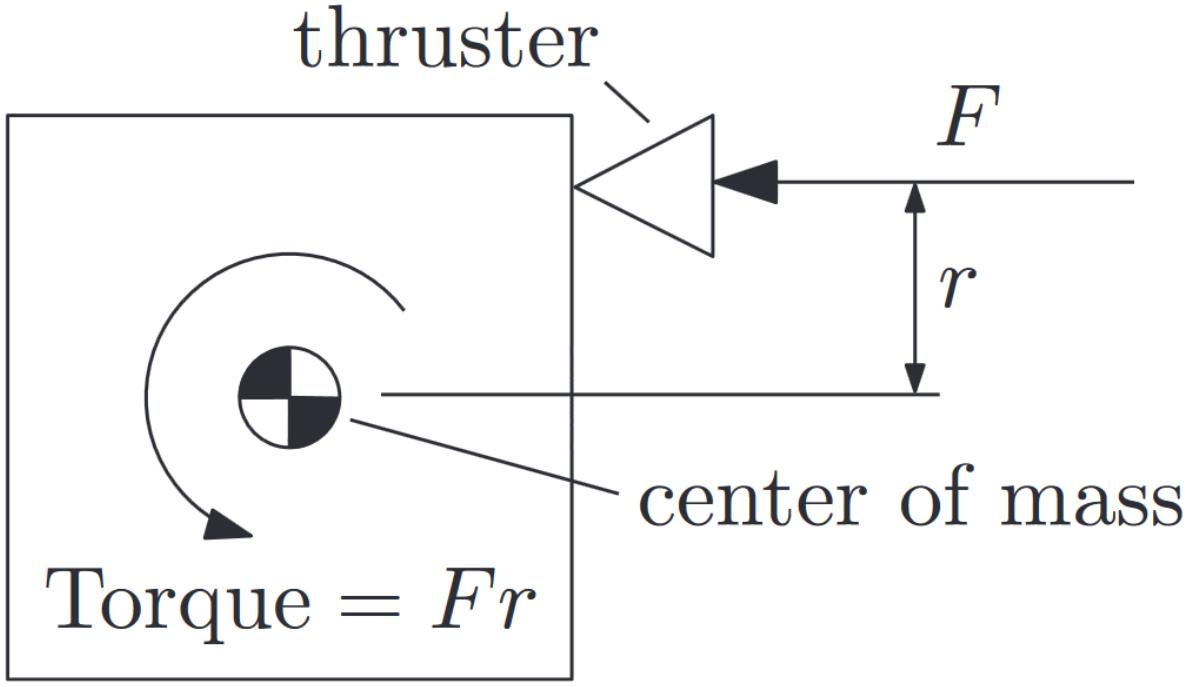
\includegraphics[width=0.5\textwidth]{images/thruster_img.png}
                \caption{Princip rada potisnika.}
                \label{fig:thruster_img}
                \end{figure}

                Zbog toga što potisnik nije u stanju generiranja sile $F$ u oba smjera (naravni i suprotni smjer), za stvaranje pozitivnog i negativnog momenta potrebno je imati dva potisnika koja su međusobno suprotno orijentirana. Sukladno tomu, za troosno upravljanje orijentacijom potrebno je imati 6 potisnika \cite{adcsKnjiga}.
            }

            \subsubsection{Magnetorkeri \engl{magnetic torquers}}{
                Magnetorkeri su aktuatori koji generiraju moment pomoću magnetske sprege lokalno generiranog magnetskog polja i magnetskog polja Zemlje. Magnetorker je u suštini zavojnica. Kao što nalaže Amperov zakon, prolaskom struje kroz namotaje zavojnice dolazi do stvaranja lokalnog magnetskog polja (magnetski dipol). Međusobnom interakcijom generiranog magnetskog dipola magnetorkera $\overrightarrow{\textbf{m}}$ i magnetskog dipola Zemlje $\overrightarrow{\textbf{b}}$ stvara se moment $\overrightarrow{\textbf{T}}$ koji je jednak:

                \begin{equation}
                    \label{eq:magnetorker_eq}
                    \overrightarrow{\textbf{T}} = \overrightarrow{\textbf{m}} \times \overrightarrow{\textbf{b}}
                \end{equation}

                Moguće je pokazati kako je vektorski produkt u jednadžbi \ref{eq:magnetorker_eq} (isto vektor) uvijek okomit na magnetski dipol Zemlje $\overrightarrow{\textbf{b}}$. Zbog toga je nemoguće generirati moment kada je položaj dipola magnetorkera usmjeren kao i dipol magnetskog polja Zemlje.

                Magnetorker omogućuje upravljanje orijentacijom samo u jedno osi, što znači da za troosno upravljanje orijentacijom tipično imamo 3 međusobno ortogonalna magnetorkera za svaku os zasebno (vidi sliku \ref{fig:magnetorquer_img}).

                \begin{figure}[htb]
                \centering
                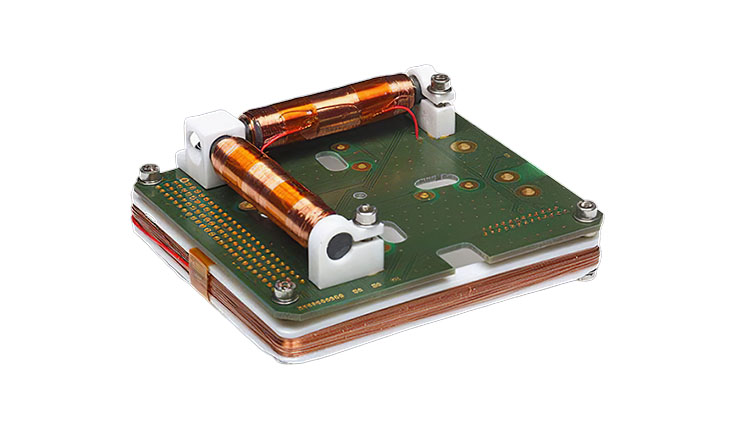
\includegraphics[width=0.7\textwidth]{images/magnetorquer_img.jpg}
                \caption{Magnetorker tvrtke NanoAvionics \cite{magnetorquer_cite}.}
                \label{fig:magnetorquer_img}
                \end{figure}

                Zbog relativno slabe jakosti Zemljinog magnetskog polja, teško je generirati momente sa dovoljnom jačinom jakosti specificirane zahtjevima, pogotovo za satelite koji posjeduju velike momente tromosti. Zbog toga najčešće se kontrola orijentacije vrši pomoću zamašnjaka (vidi kasnije poglavlje) u sprezi sa magnetorkerima iz dva razloga. Prvi razlog je već spomenuta nedovoljna jakost generiranog momenta od strane magnetorkera, i drugi razlog, problem zasićenja zamašnjaka.

                Valja skrenuti pažnju i na problem utjecaja magnetorkera na mjerenja senzora magnetskog polja. Ako prilikom korekcije orijentacije pomoću magnetorkera mjerimo magnetsko polje, doći će do magnetske interferencije magnetorkera i senzora magnetskog polja (vidi poglavlje \ref{subsubsection:troosni_magnetometar}). Samim time direktno unosimo grešku u estimaciji orijentacije. Rješenje problemu leži u tome da za vrijeme mjerenja magnetskog polja magnetorker ne vrši korekciju orijentacije \cite{adcsKnjiga}. 
            }

            \subsubsection{Zamašnjaci \engl{Momentum wheels}}{
                Zamašnjaci su mehanički uređaji koji rade na principu očuvanja kutne količine gibanja. Zamašnjak se sastoji od rotirajuće mase i elektromotora. Naime, kada elektromotorom vršimo moment u jednom smjeru, radi očuvanja kutne količine gibanja, zamašnjak će generirati jednak moment po iznosu ali u suprotnom smjeru ne bi li ukupna kutna količina gibanja satelita ostala jednaka (vidi sliku \ref{fig:zamasnjak_fig}). U nominalnom stanju, zamašnjak ne posjeduje kutnu brzinu. Zamašnjaci kao aktuatori predstavljaju najprecizniju kontrolu orijentacije \cite{adcsKnjiga}.

                \begin{figure}[htb]
                \centering
                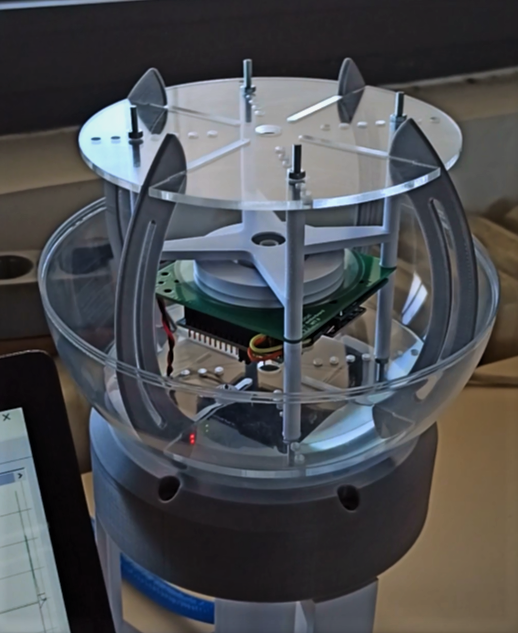
\includegraphics[width=0.7\textwidth]{images/zamasnjak.png}
                \caption{Princip rada zamašnjaka.}
                \label{fig:zamasnjak_fig}
                \end{figure}

                Problem zamašnjaka manifestira se s vremenom. Da bi objasnili problem pretpostavimo da satelitu želimo održavati jednaku orijentaciju bez obzira na vanjske utjecaje (ne ulazeći u uzroke). Svaki vanjski utjecaj (smetnja) na satelit uzrokuje generiranim momentom. Kako bismo satelitu održali jednaku orijentaciju, zamašnjakom upravljamo na način da ćemo generirati jednaki moment ali u suprotnu stranu (zamašnjak će se zarotirati u istu stranu kao i vanjski moment). Jednom kada smo pomoću zamašnjaka uveli jednaku kutnu količinu gibanja kao što ju je uvela vanjska smetnja, zamašnjaku moramo konstantno održavati kutnu brzinu. Bilo kakva promjena kutne brzine uzrokuje promjenu kutne količine gibanja odnosno promjenu orijentacije. Ako se s vremenom smetnje akumuliraju, dolazi do pojave tzv. saturacije zamašnjaka gdje se zamašnjak nastoji okretati sve većom i većom brzinom sve dok ne dosegne maksimalnu moguću kutnu brzinu. Drugi suptilni problem je taj što rotirajućem zamašnjaku stalno moramo održavati kutnu brzinu što donosi negativnu energetsku računicu. Desaturaciju zamašnjaka vršimo pomoću drugih aktuatora (npr. magnetorkera).

                Drugi problem zamašnjaka leži u činjenici da su zamašnjaci mehanički uređaji sa rotirajućim dijelovima te se očekuje da će s vremenom prestati raditi. Iz tog razloga umjesto 3 zamašnjaka za troosno upravljanje orijentacijom, uzimamo 4 zamašnjaka karakteristično položena (vidi sliku \ref{fig:cetiri_zamasnjaka}). Na taj način moguće je imati troosno upravljanje orijentacijom sa jednim zamašnjakom koji ne radi \cite{cetiriZamasnjaka}.

                \begin{figure}[htb]
                \centering
                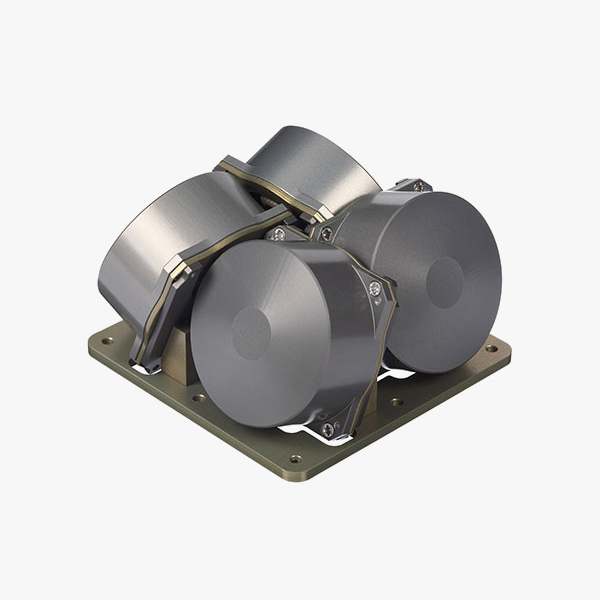
\includegraphics[width=0.5\textwidth]{images/cetiri_zamasnjaka.jpg}
                \caption{Skup od 4 zamašnjaka tvrtke NanoAvionics gdje je jedan zamašnjak redundantan \cite{cetiriZamasnjakaTvrtka}.}
                \label{fig:cetiri_zamasnjaka}
                \end{figure}
            }
        }
    }

    \section{Određivanje orijentacije}{
        \subsection{Korišteni senzori}{
            %- kako mjerimo kutnu brzinu
            %    - ziroskop
            %    - sto je ziroskop
            %    - problemi ziroskopa
        }

        \subsection{Algoritmi}{
            %- kako mozemo estimirati orijentaciju satelita
            %    - senzor fusion
            %    - navesti neke od algoritama
            %    - rekurzivni
            %    - ne rekurzivni
            %    - vidi s josipom jos neke koje je on razvijao
            %    - karla je jedan razvijala (stavi referencu)
        }
    }

    \section{Upravljanje orijentacijom}{
        \subsection{Korišteni aktuatori}{
            %- navesti aktuatore
            %- zamasnjake, magnetorqere
            %- navesti problem zasicenja zamasnjaka
        }

        \subsection{Algoritmi}{
            %- ukratko o upravljanju orijentacijom
            %- ukratko o upravljanju kutnom brzinom
            %- regulacija
            %    - navesti PID regulator kao regulator
            %    - opisati sto je PID regulator
            %    - navesti quaternion regulator kao regulator
            %        - jednadzbe
            %        - dodaj referencu na paper
        }
    }

    \section{Razvijeni sustav}{
        \subsection{Tiskana pločica i sklopovlje}{
            %- ukratko o razvijenoj plocici
            %- staviti kakvu shemu
        }

        \subsection{Izabrani senzori}{
            %- zasto koristimo IMU
            %- napisati da akcelerometar ne moze raditi u svemiru
            %- mane ziroskopa
            %    - bias
            %- mane akcelerometra
            %    - sum
            %- magnetometar
            %    - model magnetskog polja zemlje
            %        - mijenja se s vremenom
        }

        \subsection{Izabrani aktuatori}{
            %- zasto koristimo bas (stavi ime) aktuator 
            %    - a ne magnetorqer npr
            %    - za magnetorqer navesti referencu na izracun parametara koji je radio Ivan Indir
            %    - navesti karlin rad, pitaj ju sto je ona radila pa ju citiraj
        }

        \subsection{Komunikacija}{
            %- zasto koristimo bluetooth komunikaciju
            %- navest ime modula
            %- kako radi modul
            %- kako komuniciramo s njime
        }
    }
}


\chapter{Programska podrška ADCS sustava}{
    \section{Ugradbeno računalo}{
        %- koje ugradbeno racunalo koristimo
        %- zasto smo bas to odabrali
    }

    \section{Organizacija projekta}{
        %- objasniti organizaciju koda
    }
    
    \section{Korištene biblioteke}{
        %- koje biblioteke koristimo i zasto
    }

    \section{Operacijski sustav}{
        %- opisati da koristimo FreeRTOS
        %- opisati koje sve dretve imamo
        %    - za svaku dretvu napisati dijagram toka
        %    - opisati funkciju dretve
        %    - opisati vrijeme izvođenja dretvi
        %    - opisati na koji nacin dretve međusobno komuniciraju
    }

    \section{Matematički zapis orijentacije}{
        %- jednadzbe koje koristimo u SW
    }

    \section{Izabrana metoda određivanja orijentacije}{
        %- objasniti na koji nacin radimo senzor fuzion
        %    - optimal request
        %        - napisati nesto kratko o OR algoritmu
        %        - navesti referencu na svu popratnu dokumentaciju
    }

    \section{Izabrana metoda upravljanja orijentacijom}{
        %- odabrana metoda upravljanja orijentacijom
        %    - spomeni quaternion regulator
        %- odabrana metoda upravljanja kutnom brzinom
        %    - spomeni zamasnjak
        %    - pwm
        %    - spomeni PID regulator
        %    - PID regulator za kontrolu orijentacije satelita
        %        - opisati kako ga mi koristimo
        %        - ovo isto pokupi od Arduino projekta
    }

    \section{Razvoj}{
        %- objasniti koji compiler koristimo
        %- objasniti koji programski jezik koristimo
        %- objasniti da je cijeli kod na githubu
        %- broj linija koda
        %    - vidi kako to dobiti u linux-u sa nekom komandom
        %- objasniti koje sve alate koristimo prilikom razvoja SW
        %    - clang format i slicno
        %    - vscode
        %    - openocd
        %- objasniti kako debugiramo
        %- slikati graf razvoja programskog koda kroz vrijeme
    }
}

\chapter{Eksperimentalna verifikacija ADCS sustava}{
    \section{Opis sustava}{
        %- opisati zracni lezaj
        %- opisati kuglu
        %- opisati kako satelit stoji u kugli
        %- navesti reference za zracne lezaje
        %- parser
        %- program za iscrtavanje
        %- bluetooth modul za komunikaciju
        %- iscrtavanje orijentacije papirnatog avioncica u Octave programu
    }

    \section{Određivanje parametara}{
        \subsection{Kinematički model}{
            %- objasni kako smo dobili parametre
        }
    
        \subsection{PID regulator}{
            %- vidi cubesat na arduinu
            %- objasni kako smo dobili parametre PID regulatora
        }
    }

    \section{Računanje razlike trenutne i željene orijentacije}{
        \subsection{Eulerovi kutovi}{
            %- staviti formulu iz matlaba
        }

        \subsection{Kvaternioni}{
            %- staviti formule iz onog papera od josipa
        }
    }

    \section{Rezultati verifikacije}{
        %- ovo nezz
    }
}

% TODO: dodaj zakljucak
\chapter{Zaključak}{
    Ovdje ide zaključak.
}

\bibliographystyle{templates/template}
\bibliography{literatura}

% TODO: dodaj sazetak
\begin{sazetak}{
    Ovdje ide sažetak na hrvatskom jeziku.
}

% TODO: dodaj kljucne rijeci
\kljucnerijeci{Ovdje, idu, ključne, riječi, odvojene, zarezima.}
\end{sazetak}

% TODO: Dodaj naslov na engleskom
\engtitle{Put here title on english}
% TODO: Navedite Abstract
\begin{abstract}{
    Add abstract here.
}

% TODO: Navedite Keywords
\keywords{Add, keywords, here.}
\end{abstract}

\end{document}
